% Options for packages loaded elsewhere
% Options for packages loaded elsewhere
\PassOptionsToPackage{unicode}{hyperref}
\PassOptionsToPackage{hyphens}{url}
\PassOptionsToPackage{dvipsnames,svgnames,x11names}{xcolor}
%
\documentclass[
  11pt,
  letterpaper,
]{report}
\usepackage{xcolor}
\usepackage[lmargin=1in,rmargin=1in,tmargin=1in,bmargin=1in]{geometry}
\usepackage{amsmath,amssymb}
\setcounter{secnumdepth}{5}
\usepackage{iftex}
\ifPDFTeX
  \usepackage[T1]{fontenc}
  \usepackage[utf8]{inputenc}
  \usepackage{textcomp} % provide euro and other symbols
\else % if luatex or xetex
  \usepackage{unicode-math} % this also loads fontspec
  \defaultfontfeatures{Scale=MatchLowercase}
  \defaultfontfeatures[\rmfamily]{Ligatures=TeX,Scale=1}
\fi
\usepackage{lmodern}
\ifPDFTeX\else
  % xetex/luatex font selection
  \setmainfont[]{Latin Modern Roman}
  \setmonofont[]{Latin Modern Mono}
\fi
% Use upquote if available, for straight quotes in verbatim environments
\IfFileExists{upquote.sty}{\usepackage{upquote}}{}
\IfFileExists{microtype.sty}{% use microtype if available
  \usepackage[]{microtype}
  \UseMicrotypeSet[protrusion]{basicmath} % disable protrusion for tt fonts
}{}
\makeatletter
\@ifundefined{KOMAClassName}{% if non-KOMA class
  \IfFileExists{parskip.sty}{%
    \usepackage{parskip}
  }{% else
    \setlength{\parindent}{0pt}
    \setlength{\parskip}{6pt plus 2pt minus 1pt}}
}{% if KOMA class
  \KOMAoptions{parskip=half}}
\makeatother
% Make \paragraph and \subparagraph free-standing
\makeatletter
\ifx\paragraph\undefined\else
  \let\oldparagraph\paragraph
  \renewcommand{\paragraph}{
    \@ifstar
      \xxxParagraphStar
      \xxxParagraphNoStar
  }
  \newcommand{\xxxParagraphStar}[1]{\oldparagraph*{#1}\mbox{}}
  \newcommand{\xxxParagraphNoStar}[1]{\oldparagraph{#1}\mbox{}}
\fi
\ifx\subparagraph\undefined\else
  \let\oldsubparagraph\subparagraph
  \renewcommand{\subparagraph}{
    \@ifstar
      \xxxSubParagraphStar
      \xxxSubParagraphNoStar
  }
  \newcommand{\xxxSubParagraphStar}[1]{\oldsubparagraph*{#1}\mbox{}}
  \newcommand{\xxxSubParagraphNoStar}[1]{\oldsubparagraph{#1}\mbox{}}
\fi
\makeatother


\usepackage{longtable,booktabs,array}
\usepackage{calc} % for calculating minipage widths
% Correct order of tables after \paragraph or \subparagraph
\usepackage{etoolbox}
\makeatletter
\patchcmd\longtable{\par}{\if@noskipsec\mbox{}\fi\par}{}{}
\makeatother
% Allow footnotes in longtable head/foot
\IfFileExists{footnotehyper.sty}{\usepackage{footnotehyper}}{\usepackage{footnote}}
\makesavenoteenv{longtable}
\usepackage{graphicx}
\makeatletter
\newsavebox\pandoc@box
\newcommand*\pandocbounded[1]{% scales image to fit in text height/width
  \sbox\pandoc@box{#1}%
  \Gscale@div\@tempa{\textheight}{\dimexpr\ht\pandoc@box+\dp\pandoc@box\relax}%
  \Gscale@div\@tempb{\linewidth}{\wd\pandoc@box}%
  \ifdim\@tempb\p@<\@tempa\p@\let\@tempa\@tempb\fi% select the smaller of both
  \ifdim\@tempa\p@<\p@\scalebox{\@tempa}{\usebox\pandoc@box}%
  \else\usebox{\pandoc@box}%
  \fi%
}
% Set default figure placement to htbp
\def\fps@figure{htbp}
\makeatother





\setlength{\emergencystretch}{3em} % prevent overfull lines

\providecommand{\tightlist}{%
  \setlength{\itemsep}{0pt}\setlength{\parskip}{0pt}}



 


\usepackage{booktabs}
\usepackage{longtable}
\usepackage{colortbl}
\usepackage{xcolor}
\usepackage{float}
\usepackage{fancyhdr}
\usepackage{graphicx}
\usepackage{geometry}
\usepackage{enumitem}
\usepackage{tikz}
\usepackage{pgfplots}
\pgfplotsset{compat=1.18}
\definecolor{USTPurple}{HTML}{4B0082}
\definecolor{USTGray}{HTML}{58595B}
\definecolor{FINcolor}{HTML}{2E86AB}
\definecolor{BUScolor}{HTML}{A23B72}
\definecolor{OPScolor}{HTML}{F18F01}
\definecolor{ENGcolor}{HTML}{2D936C}
\definecolor{SCIcolor}{HTML}{5C4D7D}
\definecolor{COMcolor}{HTML}{E84855}
\definecolor{SOCcolor}{HTML}{1B998B}
\definecolor{AHEcolor}{HTML}{D4A373}
\definecolor{TableHeader}{HTML}{4B0082}
\definecolor{TableRowAlt}{HTML}{F5F0FF}
\pagestyle{fancy}
\fancyhf{}
\fancyhead[L]{\small\color{USTGray}Incoming → Graduating Major Analysis}
\fancyhead[R]{\small\color{USTGray}UST Career Pathways}
\fancyfoot[C]{\small\color{USTGray}\thepage}
\renewcommand{\headrulewidth}{0.4pt}
\renewcommand{\footrulewidth}{0.2pt}
\makeatletter
\@ifpackageloaded{caption}{}{\usepackage{caption}}
\AtBeginDocument{%
\ifdefined\contentsname
  \renewcommand*\contentsname{Table of contents}
\else
  \newcommand\contentsname{Table of contents}
\fi
\ifdefined\listfigurename
  \renewcommand*\listfigurename{List of Figures}
\else
  \newcommand\listfigurename{List of Figures}
\fi
\ifdefined\listtablename
  \renewcommand*\listtablename{List of Tables}
\else
  \newcommand\listtablename{List of Tables}
\fi
\ifdefined\figurename
  \renewcommand*\figurename{Figure}
\else
  \newcommand\figurename{Figure}
\fi
\ifdefined\tablename
  \renewcommand*\tablename{Table}
\else
  \newcommand\tablename{Table}
\fi
}
\@ifpackageloaded{float}{}{\usepackage{float}}
\floatstyle{ruled}
\@ifundefined{c@chapter}{\newfloat{codelisting}{h}{lop}}{\newfloat{codelisting}{h}{lop}[chapter]}
\floatname{codelisting}{Listing}
\newcommand*\listoflistings{\listof{codelisting}{List of Listings}}
\makeatother
\makeatletter
\makeatother
\makeatletter
\@ifpackageloaded{caption}{}{\usepackage{caption}}
\@ifpackageloaded{subcaption}{}{\usepackage{subcaption}}
\makeatother
\usepackage{bookmark}
\IfFileExists{xurl.sty}{\usepackage{xurl}}{} % add URL line breaks if available
\urlstyle{same}
\hypersetup{
  pdftitle={Incoming → Graduating Major Grouping Analysis},
  pdfauthor={UST Career Pathways Analysis Team},
  colorlinks=true,
  linkcolor={USTPurple},
  filecolor={Maroon},
  citecolor={Blue},
  urlcolor={USTPurple},
  pdfcreator={LaTeX via pandoc}}


\title{Incoming → Graduating Major Grouping Analysis}
\usepackage{etoolbox}
\makeatletter
\providecommand{\subtitle}[1]{% add subtitle to \maketitle
  \apptocmd{\@title}{\par {\large #1 \par}}{}{}
}
\makeatother
\subtitle{Data Visualization Design Decision Document}
\author{UST Career Pathways Analysis Team}
\date{2026-03-12}
\begin{document}
\maketitle

\renewcommand*\contentsname{Table of contents}
{
\hypersetup{linkcolor=}
\setcounter{tocdepth}{2}
\tableofcontents
}

\thispagestyle{empty}
\begin{center}
\vspace*{2cm}

{\Huge\bfseries\color{USTPurple} Incoming → Graduating Major\\[0.3cm] Grouping Analysis}

\vspace{1cm}

{\Large\color{USTGray} Data Visualization Design Decision Document}

\vspace{2cm}

{\large UST Career Pathways Analysis Team}

\vspace{0.5cm}

{\large March 12, 2026}

\vspace{3cm}

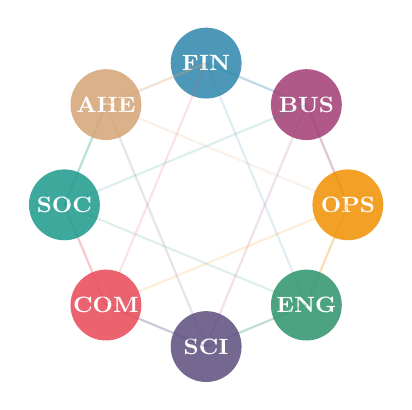
\begin{tikzpicture}
  \foreach \i/\col/\lbl in {
    0/FINcolor/FIN, 1/BUScolor/BUS, 2/OPScolor/OPS, 3/ENGcolor/ENG,
    4/SCIcolor/SCI, 5/COMcolor/COM, 6/SOCcolor/SOC, 7/AHEcolor/AHE
  } {
    \pgfmathsetmacro{\angle}{90 - \i * 45}
    \fill[\col, opacity=0.85] (\angle:1.8cm) circle (0.45cm);
    \node[white, font=\footnotesize\bfseries] at (\angle:1.8cm) {\lbl};
    \draw[\col, thick, opacity=0.3] (\angle:1.8cm) -- ({90 - mod(\i+1,8)*45}:1.8cm);
    \draw[\col, thick, opacity=0.15] (\angle:1.8cm) -- ({90 - mod(\i+3,8)*45}:1.8cm);
  }
\end{tikzpicture}

\vspace{1cm}

{\small\color{USTGray}\textit{Categorizing 91 academic majors into balanced groups\\for circos-style visualization of major migration patterns}}

\end{center}
\newpage

\tableofcontents
\newpage

\chapter*{Executive Summary}\label{executive-summary}
\addcontentsline{toc}{chapter}{Executive Summary}

This document establishes the grouping taxonomy for a new circos-style
data visualization showing how students' majors change from university
entry (incoming/declared major) to graduation (final major on record).
Unlike the existing Major → Industry circos --- which maps academic
fields to employment sectors --- this visualization maps
\textbf{academic fields to academic fields}, requiring a fundamentally
different grouping strategy.

After evaluating three candidate groupings against five weighted
criteria (visual balance, readability, academic affinity, audience
clarity, and data accommodation), we recommend \textbf{Option C: 8
Groups, Maximum Balance}. This option assigns all 91 graduating majors
to eight groups ranging from 5.1\% to 21.8\% of total students, with no
``Unclassified'' bucket and clear, intuitive group names.

\vspace{0.5cm}

\begin{center}
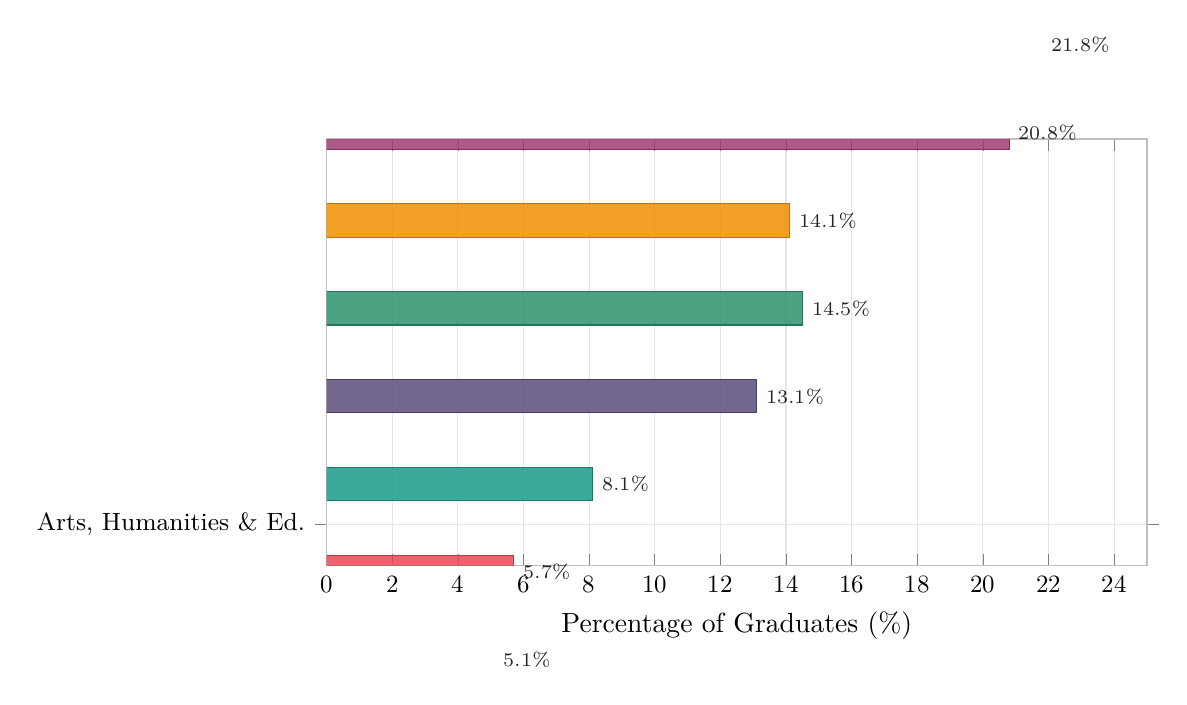
\begin{tikzpicture}
\begin{axis}[
    xbar,
    width=12cm,
    height=7cm,
    xlabel={Percentage of Graduates (\%)},
    symbolic y coords={
      {Arts, Humanities \& Ed.},
      {Communication \& Media},
      {Social Sciences},
      {Sciences \& Health},
      {Engineering \& CS},
      {Operations \& Analytics},
      {Business \& Marketing},
      {Finance \& Accounting}
    },
    ytick=data,
    y tick label style={font=\small},
    x tick label style={font=\small},
    xmin=0, xmax=25,
    bar width=12pt,
    nodes near coords={\pgfmathprintnumber\pgfplotspointmeta\%},
    nodes near coords style={font=\scriptsize, anchor=west},
    every axis plot/.append style={fill opacity=0.85},
    enlarge y limits=0.12,
    grid=major,
    grid style={gray!20},
    axis line style={gray!50},
]
\addplot[fill=AHEcolor, draw=AHEcolor!80!black] coordinates {(5.1,{Arts, Humanities \& Ed.})};
\addplot[fill=COMcolor, draw=COMcolor!80!black] coordinates {(5.7,{Communication \& Media})};
\addplot[fill=SOCcolor, draw=SOCcolor!80!black] coordinates {(8.1,{Social Sciences})};
\addplot[fill=SCIcolor, draw=SCIcolor!80!black] coordinates {(13.1,{Sciences \& Health})};
\addplot[fill=ENGcolor, draw=ENGcolor!80!black] coordinates {(14.5,{Engineering \& CS})};
\addplot[fill=OPScolor, draw=OPScolor!80!black] coordinates {(14.1,{Operations \& Analytics})};
\addplot[fill=BUScolor, draw=BUScolor!80!black] coordinates {(20.8,{Business \& Marketing})};
\addplot[fill=FINcolor, draw=FINcolor!80!black] coordinates {(21.8,{Finance \& Accounting})};
\end{axis}
\end{tikzpicture}
\end{center}

\newpage

\chapter{Visualization Objective}\label{visualization-objective}

\section{Purpose}\label{purpose}

This visualization shows how students' majors change from when they
\emph{enter} the university (incoming/declared major) to when they
\emph{graduate} (final major on record). It is designed as a
circos-style chord diagram where flows between groups represent students
who switched from one academic area to another.

\section{Target Audience}\label{target-audience}

\begin{longtable}[]{@{}
  >{\raggedright\arraybackslash}p{(\linewidth - 2\tabcolsep) * \real{0.3846}}
  >{\raggedright\arraybackslash}p{(\linewidth - 2\tabcolsep) * \real{0.6154}}@{}}
\toprule\noalign{}
\begin{minipage}[b]{\linewidth}\raggedright
Audience
\end{minipage} & \begin{minipage}[b]{\linewidth}\raggedright
What They Need
\end{minipage} \\
\midrule\noalign{}
\endhead
\bottomrule\noalign{}
\endlastfoot
Academic advisors & Understanding major migration patterns to improve
advising \\
Prospective students \& families & Seeing where students end up relative
to where they start \\
Department chairs \& deans & Retention and recruitment insights for
their programs \\
University leadership & Enrollment planning and resource allocation
data \\
\end{longtable}

\section{Key Questions This Visualization Should
Answer}\label{key-questions-this-visualization-should-answer}

\begin{enumerate}
\def\labelenumi{\arabic{enumi}.}
\tightlist
\item
  \textbf{Retention:} Which major groups retain the most students from
  entry to graduation?
\item
  \textbf{Outflow:} Where do students migrate \emph{to} when they switch
  out of a major group?
\item
  \textbf{Inflow:} Where do students migrate \emph{from} when they
  switch into a major group?
\item
  \textbf{Pipelines:} Are there predictable ``pipelines'' between
  academic areas?
\item
  \textbf{Net effect:} Which major groups are net gainers vs.~net losers
  of students?
\end{enumerate}

\chapter{Why the Existing Groupings Are
Insufficient}\label{why-the-existing-groupings-are-insufficient}

The current Major → Industry circos visualization uses \textbf{7 major
clusters} designed for career outcome analysis:

\begin{center}
\small
\begin{tabular}{ll}
\toprule
\textbf{Existing Cluster} & \textbf{Original Purpose} \\
\midrule
Arts, Languages \& Theology & Career mapping to industries \\
Business \& Management & Career mapping to industries \\
Communication \& Media & Career mapping to industries \\
Education \& Social Services & Career mapping to industries \\
Engineering \& Technology & Career mapping to industries \\
Natural \& Health Sciences & Career mapping to industries \\
Social Sciences \& Humanities & Career mapping to industries \\
\bottomrule
\end{tabular}
\end{center}

\section{Five Structural Problems}\label{five-structural-problems}

\begin{enumerate}[leftmargin=2cm, label=\textbf{Problem \arabic*.}, font=\color{USTPurple}]

\item \textbf{Both sides are majors.} The existing circos has majors on one side and industries on the other. Here, both sides are the \textit{same set} of major groups. The diagram must show flows within and between the same categories.

\item \textbf{Imbalanced sizes.} Business \& Management contains 1,758 students vs.\ Communication \& Media with 165. A single ``Business'' arc would consume over half the circos circumference, making all other flows unreadable.

\item \textbf{``Unclassified'' bucket.} The current grouping places Leadership \& Management (59 students), Mathematics (22), Statistics (18), Legal Studies (10), and others in an ``Unclassified'' category. These are legitimate majors that need proper homes.

\item \textbf{Different audience, different logic.} Career outcomes group majors by \textit{employment sector}. Major migration should group by \textit{academic affinity} — what fields are intellectually adjacent and represent likely switch paths.

\item \textbf{Incoming-only categories.} Students may enter as ``Undeclared,'' ``Exploratory,'' ``Pre-Med,'' or ``Pre-Law'' — categories that don't exist in the graduation data. The grouping must accommodate these.

\end{enumerate}

\chapter{Complete Major Inventory}\label{complete-major-inventory}

The dataset contains \textbf{91 graduating majors} across \textbf{3,201
students} (2021--2024 cohorts). Table~\ref{tbl-top20} shows the 20
largest majors, which account for 70.8\% of all graduates.

\begin{longtable}[]{@{}rlrrl@{}}
\caption{Top 20 majors by graduate count (70.8\% of
total)}\label{tbl-top20}\tabularnewline
\toprule\noalign{}
Rank & Major & Count & \% & Current Cluster \\
\midrule\noalign{}
\endfirsthead
\toprule\noalign{}
Rank & Major & Count & \% & Current Cluster \\
\midrule\noalign{}
\endhead
\bottomrule\noalign{}
\endlastfoot
1 & Financial Management & 370 & 11.6 & Business \& Management \\
2 & Marketing Management & 323 & 10.1 & Business \& Management \\
3 & Mechanical Engineering & 209 & 6.5 & Engineering \& Technology \\
4 & Accounting & 145 & 4.5 & Business \& Management \\
5 & Biology & 142 & 4.4 & Natural \& Health Sciences \\
6 & Gen Business Mgmt & 124 & 3.9 & Business \& Management \\
7 & Computer Science & 114 & 3.6 & Engineering \& Technology \\
8 & Entrepreneurship & 106 & 3.3 & Business \& Management \\
9 & Psychology & 99 & 3.1 & Social Sciences \& Humanities \\
10 & Economics & 94 & 2.9 & Business \& Management \\
11 & Actuarial Science & 86 & 2.7 & Business \& Management \\
12 & Neuroscience & 68 & 2.1 & Natural \& Health Sciences \\
13 & Exercise Science & 64 & 2.0 & Natural \& Health Sciences \\
14 & MS Operations \& SCM & 61 & 1.9 & Business \& Management \\
15 & Leadership \& Mgmt & 59 & 1.8 & \emph{Unclassified} \\
16 & Operations Management & 55 & 1.7 & Business \& Management \\
17 & Electrical Engineering & 51 & 1.6 & Engineering \& Technology \\
18 & Civil Engineering & 51 & 1.6 & Engineering \& Technology \\
19 & Human Resources Mgmt & 51 & 1.6 & Business \& Management \\
20 & Political Science & 50 & 1.6 & Social Sciences \& Humanities \\
\end{longtable}

The remaining 71 majors each represent less than 1.5\% of graduates
individually. A full inventory with group assignments is provided in the
Appendix.

\chapter{Design Constraints}\label{design-constraints}

The circos diagram imposes specific constraints on how many groups can
exist and how large each should be.

\begin{longtable}[]{@{}
  >{\raggedright\arraybackslash}p{(\linewidth - 4\tabcolsep) * \real{0.3333}}
  >{\raggedright\arraybackslash}p{(\linewidth - 4\tabcolsep) * \real{0.3611}}
  >{\raggedright\arraybackslash}p{(\linewidth - 4\tabcolsep) * \real{0.3056}}@{}}
\toprule\noalign{}
\begin{minipage}[b]{\linewidth}\raggedright
Constraint
\end{minipage} & \begin{minipage}[b]{\linewidth}\raggedright
Requirement
\end{minipage} & \begin{minipage}[b]{\linewidth}\raggedright
Rationale
\end{minipage} \\
\midrule\noalign{}
\endhead
\bottomrule\noalign{}
\endlastfoot
Maximum groups & 8--12 arcs per side & More than \textasciitilde12 makes
the circos visually cluttered \\
Size balance & No group \textgreater{} 30\% of total & Prevents any
single arc from dominating the diagram \\
Ideal range & Each group = 5--15\% & Ensures all arcs are visually
legible \\
Semantic clarity & Intuitive group names & Audience includes
non-registrar stakeholders \\
Migration logic & Group by academic affinity & Cluster majors that share
prerequisites and likely switch paths \\
Symmetry & Same taxonomy both sides & Students switch within the same
set of groups \\
Incoming accommodation & Reserve slots & Incoming side may include
Undeclared, Pre-Professional, etc. \\
\end{longtable}

\chapter{Proposed Groupings}\label{proposed-groupings}

Three candidate groupings were evaluated, each optimizing for different
priorities.

\section{Option A: 10 Academic
Divisions}\label{option-a-10-academic-divisions}

This grouping prioritizes \textbf{academic granularity} with
fine-grained distinctions between fields.

\begin{longtable}[]{@{}rlrr@{}}
\caption{Option A --- 10 Academic
Divisions}\label{tbl-optionA}\tabularnewline
\toprule\noalign{}
\# & Group Name & Count & \% \\
\midrule\noalign{}
\endfirsthead
\toprule\noalign{}
\# & Group Name & Count & \% \\
\midrule\noalign{}
\endhead
\bottomrule\noalign{}
\endlastfoot
1 & Finance \& Accounting & 603 & 18.8 \\
2 & Marketing \& Business Operations & 667 & 20.8 \\
3 & Management \& Analytics & 451 & 14.1 \\
4 & Engineering & 347 & 10.8 \\
5 & Computer Science \& Math & 138 & 4.3 \\
6 & Biological \& Health Sciences & 355 & 11.1 \\
7 & Physical \& Environmental Sciences & 64 & \textbf{2.0} \\
8 & Communication \& Media & 170 & 5.3 \\
9 & Social Sciences \& Public Affairs & 260 & 8.1 \\
10 & Arts, Humanities \& Languages & 163 & 5.1 \\
\end{longtable}

\textbf{Strengths:} Fine-grained academic distinctions; all previously
unclassified majors assigned; Business split into three logical
sub-groups.

\textbf{Weaknesses:} Physical \& Environmental Sciences is only 2.0\%
(would produce a nearly invisible arc); Computer Science \& Math at
4.3\% is also marginal; 10 arcs creates visual density.

\section{Option B: 8 Balanced
Divisions}\label{option-b-8-balanced-divisions}

This grouping consolidates to \textbf{8 groups} by merging small
categories.

\begin{longtable}[]{@{}rlrr@{}}
\caption{Option B --- 8 Balanced
Divisions}\label{tbl-optionB}\tabularnewline
\toprule\noalign{}
\# & Group Name & Count & \% \\
\midrule\noalign{}
\endfirsthead
\toprule\noalign{}
\# & Group Name & Count & \% \\
\midrule\noalign{}
\endhead
\bottomrule\noalign{}
\endlastfoot
1 & Finance \& Accounting & 697 & 21.8 \\
2 & Business \& Marketing & 667 & 20.8 \\
3 & Operations, Analytics \& Law & 451 & 14.1 \\
4 & Engineering \& Computer Science & 463 & 14.5 \\
5 & Biological \& Health Sciences & 355 & 11.1 \\
6 & Physical \& Environmental Sciences & 64 & \textbf{2.0} \\
7 & Communication, Media \& Writing & 184 & 5.7 \\
8 & Social Sciences, Humanities \& Education & 423 & 13.2 \\
\end{longtable}

\textbf{Strengths:} 8 arcs for cleaner visual; Engineering + CS merged
(realistic switch path); most groups 11--22\%.

\textbf{Weaknesses:} Physical \& Environmental Sciences still at 2.0\%;
Group 8 is a catch-all mixing social sciences, humanities, arts,
languages, and education.

\section{Option C: 8 Groups, Maximum Balance
(Recommended)}\label{sec-optionC}

Optimized to eliminate all sub-5\% groups except those that are
semantically distinct.

\begin{longtable}[]{@{}
  >{\raggedleft\arraybackslash}p{(\linewidth - 10\tabcolsep) * \real{0.0952}}
  >{\raggedright\arraybackslash}p{(\linewidth - 10\tabcolsep) * \real{0.2857}}
  >{\centering\arraybackslash}p{(\linewidth - 10\tabcolsep) * \real{0.1905}}
  >{\raggedleft\arraybackslash}p{(\linewidth - 10\tabcolsep) * \real{0.1667}}
  >{\raggedleft\arraybackslash}p{(\linewidth - 10\tabcolsep) * \real{0.0952}}
  >{\raggedright\arraybackslash}p{(\linewidth - 10\tabcolsep) * \real{0.1667}}@{}}
\caption{Option C --- 8 Groups, Maximum Balance
(Recommended)}\label{tbl-optionC}\tabularnewline
\toprule\noalign{}
\begin{minipage}[b]{\linewidth}\raggedleft
\#
\end{minipage} & \begin{minipage}[b]{\linewidth}\raggedright
Group Name
\end{minipage} & \begin{minipage}[b]{\linewidth}\centering
Abbrev
\end{minipage} & \begin{minipage}[b]{\linewidth}\raggedleft
Count
\end{minipage} & \begin{minipage}[b]{\linewidth}\raggedleft
\%
\end{minipage} & \begin{minipage}[b]{\linewidth}\raggedright
Color
\end{minipage} \\
\midrule\noalign{}
\endfirsthead
\toprule\noalign{}
\begin{minipage}[b]{\linewidth}\raggedleft
\#
\end{minipage} & \begin{minipage}[b]{\linewidth}\raggedright
Group Name
\end{minipage} & \begin{minipage}[b]{\linewidth}\centering
Abbrev
\end{minipage} & \begin{minipage}[b]{\linewidth}\raggedleft
Count
\end{minipage} & \begin{minipage}[b]{\linewidth}\raggedleft
\%
\end{minipage} & \begin{minipage}[b]{\linewidth}\raggedright
Color
\end{minipage} \\
\midrule\noalign{}
\endhead
\bottomrule\noalign{}
\endlastfoot
1 & Finance \& Accounting & FIN & 697 & 21.8 &
\textcolor{FINcolor}{$\blacksquare$} \\
2 & Business \& Marketing & BUS & 667 & 20.8 &
\textcolor{BUScolor}{$\blacksquare$} \\
3 & Operations, Analytics \& Law & OPS & 451 & 14.1 &
\textcolor{OPScolor}{$\blacksquare$} \\
4 & Engineering \& Computer Science & ENG & 463 & 14.5 &
\textcolor{ENGcolor}{$\blacksquare$} \\
5 & Sciences \& Health & SCI & 419 & 13.1 &
\textcolor{SCIcolor}{$\blacksquare$} \\
6 & Communication, Media \& Writing & COM & 184 & 5.7 &
\textcolor{COMcolor}{$\blacksquare$} \\
7 & Social Sciences \& Public Affairs & SOC & 260 & 8.1 &
\textcolor{SOCcolor}{$\blacksquare$} \\
8 & Arts, Humanities \& Education & AHE & 163 & 5.1 &
\textcolor{AHEcolor}{$\blacksquare$} \\
\end{longtable}

\subsection{Key Design Decisions in Option
C}\label{key-design-decisions-in-option-c}

\begin{itemize}[leftmargin=1.5cm]
\item[\textcolor{SCIcolor}{$\blacktriangleright$}] \textbf{All sciences merged.} Biological, physical, environmental, and health sciences are unified into one ``Sciences \& Health'' group (13.1\%). This eliminates the 2.0\% sliver and reflects that Bio $\leftrightarrow$ Chem $\leftrightarrow$ Physics switches are common.

\item[\textcolor{FINcolor}{$\blacktriangleright$}] \textbf{Business split three ways.} Business-related majors constitute 54\% of graduates. A single ``Business'' arc would dominate the circos. Three groups (FIN, BUS, OPS) distribute this mass while preserving meaningful academic boundaries.

\item[\textcolor{ENGcolor}{$\blacktriangleright$}] \textbf{CS placed with Engineering.} Computer Science $\leftrightarrow$ Computer Engineering $\leftrightarrow$ Electrical Engineering is one of the most common switch paths. Grouping them together captures this affinity.

\item[\textcolor{COMcolor}{$\blacktriangleright$}] \textbf{English placed with Communication.} English, Creative Writing, and Professional Writing share more migration affinity with Communication and Journalism than with Humanities.

\item[\textcolor{AHEcolor}{$\blacktriangleright$}] \textbf{Education placed with Arts \& Humanities.} Education majors (Elementary Ed, Secondary Ed, Music Ed) have strong academic ties to their subject-area humanities and arts programs.
\end{itemize}

\subsection{Size Distribution
Visualization}\label{size-distribution-visualization}

\begin{center}
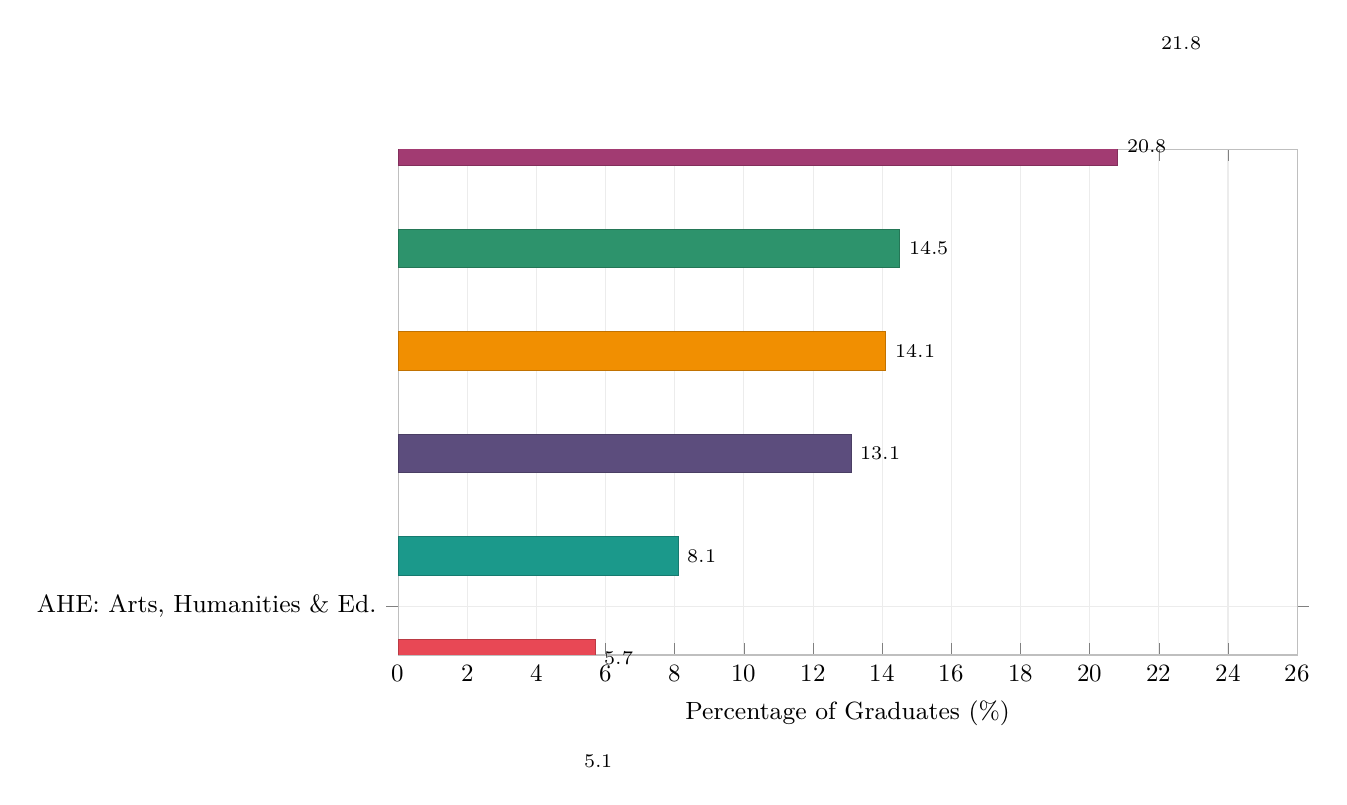
\begin{tikzpicture}
\begin{axis}[
    xbar,
    width=13cm,
    height=8cm,
    xlabel={\small Percentage of Graduates (\%)},
    symbolic y coords={
      {AHE: Arts, Humanities \& Ed.},
      {COM: Communication \& Media},
      {SOC: Social Sciences},
      {SCI: Sciences \& Health},
      {OPS: Operations \& Analytics},
      {ENG: Engineering \& CS},
      {BUS: Business \& Marketing},
      {FIN: Finance \& Accounting}
    },
    ytick=data,
    y tick label style={font=\small},
    x tick label style={font=\small},
    xmin=0, xmax=26,
    bar width=14pt,
    nodes near coords,
    nodes near coords style={font=\scriptsize, anchor=west, /pgf/number format/.cd, fixed, precision=1, /tikz/.cd},
    point meta=explicit,
    enlarge y limits=0.12,
    grid=major,
    grid style={gray!15},
    axis line style={gray!50},
    title style={font=\bfseries, at={(0.5,1.05)}},
]
\addplot[fill=AHEcolor, draw=AHEcolor!80!black] coordinates {(5.1,{AHE: Arts, Humanities \& Ed.}) [5.1]};
\addplot[fill=COMcolor, draw=COMcolor!80!black] coordinates {(5.7,{COM: Communication \& Media}) [5.7]};
\addplot[fill=SOCcolor, draw=SOCcolor!80!black] coordinates {(8.1,{SOC: Social Sciences}) [8.1]};
\addplot[fill=SCIcolor, draw=SCIcolor!80!black] coordinates {(13.1,{SCI: Sciences \& Health}) [13.1]};
\addplot[fill=OPScolor, draw=OPScolor!80!black] coordinates {(14.1,{OPS: Operations \& Analytics}) [14.1]};
\addplot[fill=ENGcolor, draw=ENGcolor!80!black] coordinates {(14.5,{ENG: Engineering \& CS}) [14.5]};
\addplot[fill=BUScolor, draw=BUScolor!80!black] coordinates {(20.8,{BUS: Business \& Marketing}) [20.8]};
\addplot[fill=FINcolor, draw=FINcolor!80!black] coordinates {(21.8,{FIN: Finance \& Accounting}) [21.8]};
\end{axis}
\end{tikzpicture}
\end{center}

\chapter{Decision Matrix}\label{decision-matrix}

Each option was scored against five weighted criteria on a 1--3 scale.

\renewcommand{\arraystretch}{1.3}
\begin{center}
\small
\begin{tabular}{p{4cm}ccc}
\toprule
\textbf{Criteria (Weight)} & \textbf{Option A} & \textbf{Option B} & \textbf{Option C} \\
\midrule
Visual balance (30\%) & 2 & 2 & \textbf{3} \\
{\scriptsize \textit{No group < 5\%}} & {\scriptsize Phys/Env = 2\%} & {\scriptsize Phys/Env = 2\%} & {\scriptsize Min = 5.1\%} \\[4pt]
Readability (25\%) & 2 & 3 & \textbf{3} \\
{\scriptsize \textit{Optimal arc count}} & {\scriptsize 10 arcs, dense} & {\scriptsize 8 arcs, clean} & {\scriptsize 8 arcs, clean} \\[4pt]
Academic affinity (20\%) & 3 & 2 & \textbf{3} \\
{\scriptsize \textit{Coherent groupings}} & {\scriptsize Fine-grained} & {\scriptsize Catch-all group} & {\scriptsize All coherent} \\[4pt]
Audience clarity (15\%) & 2 & 3 & \textbf{3} \\
{\scriptsize \textit{Intuitive for stakeholders}} & {\scriptsize Too many to scan} & {\scriptsize Easy to understand} & {\scriptsize Easy to understand} \\[4pt]
Incoming data (10\%) & 3 & 3 & \textbf{3} \\
{\scriptsize \textit{Accommodates Undeclared}} & {\scriptsize Room available} & {\scriptsize Room available} & {\scriptsize Room available} \\
\midrule
\textbf{Weighted Score} & \textbf{2.30} & \textbf{2.55} & \textbf{2.85} \\
\bottomrule
\end{tabular}
\end{center}

\vspace{0.5cm}
\begin{center}
\fbox{\Large\bfseries\color{USTPurple} Recommendation: Option C — 8 Groups, Maximum Balance}
\end{center}

\chapter{Complete Mapping Reference (Option C)}\label{sec-mapping}

\section{Finance \& Accounting (FIN) --- 697 graduates,
21.8\%}\label{finance-accounting-fin-697-graduates-21.8}

\begin{longtable}[]{@{}lrl@{}}
\toprule\noalign{}
Major & Count & Rationale \\
\midrule\noalign{}
\endhead
\bottomrule\noalign{}
\endlastfoot
Financial Management & 370 & Core finance \\
Accounting & 145 & Core finance \\
Actuarial Science & 86 & Quantitative finance \\
Economics & 94 & Economics → Finance is the most common switch path \\
Risk Management and Insurance & 2 & Financial risk specialization \\
\end{longtable}

\section{Business \& Marketing (BUS) --- 667 graduates,
20.8\%}\label{business-marketing-bus-667-graduates-20.8}

\begin{longtable}[]{@{}lrl@{}}
\toprule\noalign{}
Major & Count & Rationale \\
\midrule\noalign{}
\endhead
\bottomrule\noalign{}
\endlastfoot
Marketing Management & 323 & Core business/marketing \\
Gen Business Mgmt & 124 & General business \\
Entrepreneurship & 106 & Business venture creation \\
Bus Admin - Communication & 31 & Business administration track \\
International Business & 21 & Business specialization \\
Real Estate Studies & 37 & Business specialization \\
Business Communication & 3 & Business administration track \\
Family Business & 1 & Business specialization \\
MS Business Analytics & 1 & Graduate business track \\
\end{longtable}

\section{Operations, Analytics \& Law (OPS) --- 451 graduates,
14.1\%}\label{operations-analytics-law-ops-451-graduates-14.1}

\begin{longtable}[]{@{}lrl@{}}
\toprule\noalign{}
Major & Count & Rationale \\
\midrule\noalign{}
\endhead
\bottomrule\noalign{}
\endlastfoot
MS Operations \& Supply Chain Mgmt & 61 & Operations discipline \\
Operations Management & 55 & Operations discipline \\
Human Resources Management & 51 & Organizational management \\
Leadership \& Management & 59 & Organizational management \\
Data Analytics & 29 & Quantitative/analytical \\
Statistics & 18 & Often switches with Data Analytics \\
Mathematics & 22 & Applied math → analytics pipeline \\
Law \& Compliance & 30 & Regulatory/professional \\
Legal Studies & 10 & Regulatory/professional \\
\end{longtable}

\noindent\textit{Note: This group absorbs all previously ``Unclassified'' quantitative and professional majors.}

\section{Engineering \& Computer Science (ENG) --- 463 graduates,
14.5\%}\label{engineering-computer-science-eng-463-graduates-14.5}

\begin{longtable}[]{@{}lrl@{}}
\toprule\noalign{}
Major & Count & Rationale \\
\midrule\noalign{}
\endhead
\bottomrule\noalign{}
\endlastfoot
Mechanical Engineering & 209 & Core engineering \\
Electrical Engineering & 51 & Core engineering \\
Civil Engineering & 51 & Core engineering \\
Computer Engineering & 36 & Engineering/CS overlap \\
Computer Science & 114 & CS ↔ Engineering frequent switch \\
Comp Science BS (Master Track) & 1 & CS variant \\
Quant Methods - Computer Sci & 1 & CS variant \\
\end{longtable}

\section{Sciences \& Health (SCI) --- 419 graduates,
13.1\%}\label{sciences-health-sci-419-graduates-13.1}

\begin{longtable}[]{@{}lrl@{}}
\toprule\noalign{}
Major & Count & Rationale \\
\midrule\noalign{}
\endhead
\bottomrule\noalign{}
\endlastfoot
Biology & 142 & Core biological science \\
Neuroscience & 68 & Biological science \\
Biochemistry & 41 & Biological science \\
Biology of Global Health & 17 & Health-focused biology \\
Exercise Science & 64 & Health science \\
Public Health & 26 & Health science \\
Health Promotion \& Wellness & 9 & Health science \\
Nursing & 1 & Health profession \\
Environmental Sci (Biology) & 9 & Environmental/biological \\
Chemistry & 24 & Physical science \\
Physics & 6 & Physical science \\
Geology & 9 & Earth science \\
Environmental Studies & 12 & Environmental science \\
Environmental Sci (Geoscience) & 9 & Environmental science \\
Environmental Sci (Chemistry) & 1 & Environmental science \\
Environmental Science & 2 & Environmental science \\
Geography & 1 & Earth/environmental \\
Geography - Geo Info Sys (GIS) & 5 & Applied geography \\
\end{longtable}

\noindent\textit{Note: Merging biological, physical, and environmental sciences eliminates the 2.0\% sliver from Options A and B, reflecting natural Bio $\leftrightarrow$ Chem $\leftrightarrow$ Physics migration paths.}

\section{Communication, Media \& Writing (COM) --- 184 graduates,
5.7\%}\label{communication-media-writing-com-184-graduates-5.7}

\begin{longtable}[]{@{}lrl@{}}
\toprule\noalign{}
Major & Count & Rationale \\
\midrule\noalign{}
\endhead
\bottomrule\noalign{}
\endlastfoot
Communication Studies & 23 & Core communication \\
Strategic Comm: Ad and PR & 22 & Communication specialization \\
COJO Strategic Communications & 20 & Communication specialization \\
COJO Persuasion/Soc Influence & 7 & Communication specialization \\
COJO Interpersonal Comm & 1 & Communication specialization \\
Strategic Communication & 1 & Communication specialization \\
Communication and Journalism & 2 & Communication/journalism \\
Digital Media Arts & 25 & Media production \\
Journalism & 17 & Journalism/media \\
COJO Journalism & 12 & Journalism/media \\
COJO Creative Multimedia & 9 & Media production \\
English - Creative Writing & 21 & Writing → media pipeline \\
English & 14 & English → writing/media pipeline \\
English - Professional Writing & 9 & Writing specialization \\
\end{longtable}

\section{Social Sciences \& Public Affairs (SOC) --- 260 graduates,
8.1\%}\label{social-sciences-public-affairs-soc-260-graduates-8.1}

\begin{longtable}[]{@{}lrl@{}}
\toprule\noalign{}
Major & Count & Rationale \\
\midrule\noalign{}
\endhead
\bottomrule\noalign{}
\endlastfoot
Psychology & 99 & Core social science \\
Political Science & 50 & Core social science \\
Criminal Justice & 24 & Applied social science \\
Social Work & 26 & Applied social science \\
Social Work Advanced Standing & 2 & Applied social science \\
Justice \& Peace Studies & 11 & Social justice focus \\
Sociology & 11 & Core social science \\
Family Studies & 8 & Applied social science \\
Individualized & 10 & Often social-science oriented \\
Intl Studies - Pol Sci & 10 & Political/international studies \\
Intl Studies - Economics & 4 & International studies \\
Intl Studies - History & 3 & International studies \\
\end{longtable}

\section{Arts, Humanities \& Education (AHE) --- 163 graduates,
5.1\%}\label{arts-humanities-education-ahe-163-graduates-5.1}

\begin{longtable}[]{@{}lrl@{}}
\toprule\noalign{}
Major & Count & Rationale \\
\midrule\noalign{}
\endhead
\bottomrule\noalign{}
\endlastfoot
Philosophy & 39 & Core humanities \\
History & 18 & Core humanities \\
Classical Civilization & 2 & Humanities \\
Catholic Studies & 30 & Theology/humanities \\
Theology & 3 & Theology/humanities \\
Music - Business & 11 & Arts \\
Music & 3 & Arts \\
Music - Performance & 2 & Arts \\
Art History & 2 & Arts/humanities \\
Spanish Cultural/Literary St. & 5 & Languages \\
Spanish Linguistics/Lang. St. & 3 & Languages \\
French & 3 & Languages \\
German & 1 & Languages \\
K-12 Music Education & 3 & Education/arts \\
K-12 World Lang. \& Cultures & 1 & Education/languages \\
Elementary Education (K-6) & 32 & Education \\
Middle/Secondary Education & 14 & Education \\
\end{longtable}

\section{Incoming-Only Groups (When Data
Available)}\label{incoming-only-groups-when-data-available}

These groups will appear only on the \textbf{incoming side} of the
circos diagram:

\begin{itemize}
\item \textbf{Undeclared / Exploratory} — Students who enter without a declared major
\item \textbf{Pre-Professional} — Pre-Med, Pre-Law, Pre-Dental, and similar tracks that do not correspond to a graduating major
\end{itemize}

\chapter{Open Questions \& Next Steps}\label{open-questions-next-steps}

\section{Data Requirements}\label{data-requirements}

\begin{enumerate}
\item \textbf{Incoming major data:} What major did each student declare upon entry?
\item \textbf{Student-level linkage:} Same student's incoming major $\leftrightarrow$ graduating major
\item \textbf{Cohort scope:} Which graduation years? Same 2021--2024 window?
\item \textbf{Undeclared handling:} Should ``Undeclared'' be its own group, or should those students be counted in their eventual graduating group only?
\end{enumerate}

\section{Pending Design Decisions}\label{pending-design-decisions}

\begin{longtable}[]{@{}
  >{\raggedright\arraybackslash}p{(\linewidth - 2\tabcolsep) * \real{0.2564}}
  >{\raggedright\arraybackslash}p{(\linewidth - 2\tabcolsep) * \real{0.7436}}@{}}
\toprule\noalign{}
\begin{minipage}[b]{\linewidth}\raggedright
Decision
\end{minipage} & \begin{minipage}[b]{\linewidth}\raggedright
Options Under Consideration
\end{minipage} \\
\midrule\noalign{}
\endhead
\bottomrule\noalign{}
\endlastfoot
Color palette & Reuse existing circos palette, or create new 8-color
palette? \\
Self-loops & Show students who stay in the same group? (may dominate
flows) \\
Minimum threshold & Ignore flows with fewer than \(n\) students? (e.g.,
\(n = 5\)) \\
Value display & Absolute counts vs.~percentages vs.~both? \\
Label strategy & Abbreviated labels on arcs with full names in
legend? \\
\end{longtable}

\section{Implementation Roadmap}\label{implementation-roadmap}

\begin{enumerate}
\item Obtain incoming-major-to-graduating-major paired data
\item Apply this grouping taxonomy to both incoming and graduating sides
\item Build flow matrix (\texttt{group\_incoming} $\times$ \texttt{group\_graduating})
\item Generate karyotype and links files for Circos
\item Render initial visualization and iterate on visual design
\item Validate with stakeholders and refine groupings if needed
\end{enumerate}

\appendix
\renewcommand{\thesection}{\Alph{section}}

\chapter{Complete Major-to-Group Assignment
Table}\label{sec-appendix-full}

The following table lists all 91 majors with their assigned group code,
sorted alphabetically.

\small
\renewcommand{\arraystretch}{1.1}

\begin{longtable}[]{@{}lcr@{}}
\toprule\noalign{}
Major & Group & Count \\
\midrule\noalign{}
\endhead
\bottomrule\noalign{}
\endlastfoot
Accounting & FIN & 145 \\
Actuarial Science & FIN & 86 \\
Art History & AHE & 2 \\
Biochemistry & SCI & 41 \\
Biology & SCI & 142 \\
Biology of Global Health & SCI & 17 \\
Bus Admin - Communication & BUS & 31 \\
Business Communication & BUS & 3 \\
Catholic Studies & AHE & 30 \\
Chemistry & SCI & 24 \\
Civil Engineering & ENG & 51 \\
Classical Civilization & AHE & 2 \\
COJO Creative Multimedia & COM & 9 \\
COJO Interpersonal Comm & COM & 1 \\
COJO Journalism & COM & 12 \\
COJO Persuasion/Soc Influence & COM & 7 \\
COJO Strategic Communications & COM & 20 \\
Comm. and Journalism & COM & 2 \\
Communication Studies & COM & 23 \\
Comp Science BS (Master Track) & ENG & 1 \\
Computer Engineering & ENG & 36 \\
Computer Science & ENG & 114 \\
Criminal Justice & SOC & 24 \\
Data Analytics & OPS & 29 \\
Digital Media Arts & COM & 25 \\
Economics & FIN & 94 \\
Electrical Engineering & ENG & 51 \\
Elementary Education (K-6) & AHE & 32 \\
English & COM & 14 \\
English - Creative Writing & COM & 21 \\
English - Professional Writing & COM & 9 \\
Entrepreneurship & BUS & 106 \\
Environmental Sci (Biology) & SCI & 9 \\
Environmental Sci (Chemistry) & SCI & 1 \\
Environmental Sci (Geoscience) & SCI & 9 \\
Environmental Science & SCI & 2 \\
Environmental Studies & SCI & 12 \\
Exercise Science & SCI & 64 \\
Family Business & BUS & 1 \\
Family Studies & SOC & 8 \\
Financial Management & FIN & 370 \\
French & AHE & 3 \\
Gen Business Mgmt & BUS & 124 \\
Geography & SCI & 1 \\
Geography - GIS & SCI & 5 \\
Geology & SCI & 9 \\
German & AHE & 1 \\
Health Promotion \& Wellness & SCI & 9 \\
History & AHE & 18 \\
Human Resources Mgmt & OPS & 51 \\
Individualized & SOC & 10 \\
International Business & BUS & 21 \\
Intl Studies - Economics & SOC & 4 \\
Intl Studies - History & SOC & 3 \\
Intl Studies - Pol Sci & SOC & 10 \\
Journalism & COM & 17 \\
Justice \& Peace Studies & SOC & 11 \\
K-12 Music Education & AHE & 3 \\
K-12 World Lang. \& Cultures & AHE & 1 \\
Law \& Compliance & OPS & 30 \\
Leadership \& Management & OPS & 59 \\
Legal Studies & OPS & 10 \\
Marketing Management & BUS & 323 \\
Mathematics & OPS & 22 \\
Mechanical Engineering & ENG & 209 \\
Middle/Secondary Education & AHE & 14 \\
MS Business Analytics & BUS & 1 \\
MS Operations \& SCM & OPS & 61 \\
Music & AHE & 3 \\
Music - Business & AHE & 11 \\
Music - Performance & AHE & 2 \\
Neuroscience & SCI & 68 \\
Nursing & SCI & 1 \\
Operations Management & OPS & 55 \\
Philosophy & AHE & 39 \\
Physics & SCI & 6 \\
Political Science & SOC & 50 \\
Psychology & SOC & 99 \\
Public Health & SCI & 26 \\
Quant Methods - Computer Sci & ENG & 1 \\
Real Estate Studies & BUS & 37 \\
Risk Management \& Insurance & FIN & 2 \\
Social Work & SOC & 26 \\
Social Work Adv. Standing & SOC & 2 \\
Sociology & SOC & 11 \\
Spanish Cultural/Literary St. & AHE & 5 \\
Spanish Linguistics/Lang. St. & AHE & 3 \\
Statistics & OPS & 18 \\
Strategic Comm: Ad and PR & COM & 22 \\
Strategic Communication & COM & 1 \\
Theology & AHE & 3 \\
\end{longtable}




\end{document}
